\documentclass[11pt]{article}

\RequirePackage[letterpaper,left=1.0in,top=1.0in,bottom=1.0in,right=1.0in,nohead,nofoot]{geometry}

% Load packages
\usepackage{times}
\usepackage{url}  % Formatting web addresses
\usepackage{ifthen}  % Conditional
\usepackage{multicol}   %Columns
\usepackage[utf8]{inputenc} %unicode support
\usepackage{amsmath}
\usepackage{amssymb}
\usepackage{epsfig}
\usepackage{epstopdf}
\usepackage{graphicx}
\usepackage[font=scriptsize,labelfont=bf]{caption}
\usepackage{setspace}
%\usepackage{longtable}
\usepackage{colortbl}
%\usepackage{palatino,lettrine}
%\usepackage{times}
%\usepackage[applemac]{inputenc} %applemac support if unicode package fails
%\usepackage[latin1]{inputenc} %UNIX support if unicode package fails
\usepackage[wide]{sidecap}
%\usepackage[authoryear,round,comma,sort&compress]{natbib}
%\usepackage[round,sort,comma,numbers,sort&compress]{natbib}
%\usepackage[authoryear,round]{natbib}
\usepackage{supertabular}
\usepackage{simplemargins}
\usepackage{fullpage}
\usepackage{comment}
\usepackage{lineno}
%\usepackage{chicago}
\usepackage{textcomp}
\usepackage{multirow}
\usepackage{amsmath}
\usepackage[linesnumbered,lined,boxed,commentsnumbered]{algorithm2e}
\DeclareMathOperator*{\argmin}{\arg\!\min}

\usepackage{algorithm2e}
\usepackage{algpseudocode}
%\usepackage[space]{cite}
\urlstyle{rm}

%\textwidth = 6.50 in
%\textheight = 9.5 in
%\oddsidemargin =  0.0 in
%\evensidemargin = 0.0 in
%\topmargin = -0.50 in
%\headheight = 0.0 in
%\headsep = 0.25 in
%\parskip = 0.15in
%\linespread{1.75}

%\bibliographystyle{chicago}
\bibliographystyle{plos2009}
\usepackage[square,sort,comma,numbers,sort&compress]{natbib}
\usepackage{wrapfig}

\makeatletter
\renewcommand\subsection{\@startsection
	{subsection}{2}{0mm}
	{-0.05in}
	{-0.5\baselineskip}
	{\normalfont\normalsize\bfseries}}
\renewcommand\subsubsection{\@startsection
	{subsubsection}{2}{0mm}
	{-0.05in}
	{-0.5\baselineskip}
	{\normalfont\normalsize\bfseries}}
\renewcommand\section{\@startsection
	{subsection}{2}{0mm}
	{-0.2in}
	{0.05\baselineskip}
	{\normalfont\large\bfseries}}
\renewcommand\paragraph{\@startsection
  {paragraph}{2}{0mm}
  {-0.05in}
  {-0.5\baselineskip}
  {\normalfont\normalsize\itshape}}
\makeatother

%Review style settings
%\newenvironment{bmcformat}{\begin{raggedright}\baselineskip20pt\sloppy\setboolean{publ}{false}}{\end{raggedright}\baselineskip20pt\sloppy}

%Publication style settings

% Single space'd bib -
\setlength\bibsep{0pt}

\renewcommand{\rmdefault}{phv}\renewcommand{\sfdefault}{phv}
\newcommand{\norm}[1]{\left\lVert#1\right\rVert}

% Change the number format in the ref list -
\renewcommand{\bibnumfmt}[1]{#1.}

% Change Figure to Fig.
\renewcommand{\figurename}{Fig.}
\everymath{\displaystyle}
\begin{document}
%%%%%%%%%%%%%%%%%%%%%%%%%%%%%%%%%%%%%%%%%%%%%%%%%%%%%%%%%%%%%%%%%%%%%
% TITLE PAGE
%%%%%%%%%%%%%%%%%%%%%%%%%%%%%%%%%%%%%%%%%%%%%%%%%%%%%%%%%%%%%%%%%%%%%
\begin{titlepage}
  \begin{center}
    \vspace*{\stretch{0.8}}
    {\LARGE{Towards a Personalized, State Aware Model of Trauma}}\par
    \vspace{5em}
    { \Large{Rachel LeCover} \\
    \vspace{1em}
    { \large{Advisor: Jeffrey D. Varner}}\par
     \vspace{3em}
    { \large{Qualifying Examination}}\par
     \vspace{1em}
    { \large{August 1, 2016}}\par
    \begin{figure}[h]
    \vspace{3em}
       \centering
       
\includegraphics[width=0.7\textwidth]{figures/CULogo187}
       \end{figure}
    \vspace{2em} \large{ \textit{School of Chemical and Biomolecular Engineering \\ \vspace{0.5em} Cornell University, Ithaca, NY}}}\par
    \vspace{3em}
  \end{center}
\end{titlepage}
\pagebreak
%%%%%%%%%%%%%%%%%%%%%%%%%%%%%%%%%%%%%%%%%%%%%%%%%%%%%%%%%%%%%%%%%%%%%
% INTRODUCTION
%%%%%%%%%%%%%%%%%%%%%%%%%%%%%%%%%%%%%%%%%%%%%%%%%%%%%%%%%%%%%%%%%%%%%
\setcounter{page}{1}
% \section*{Abstract}
% We propose the development of a personalized, state aware, high fidelity model of traumatic injury.
% The proposed model will capture both the physical and biochemical aspects of trauma.
% We have constructed an eight compartment body, with a small wound connected to the arterial compartment.
% Through a heart rate prediction model, we allowed the volumes of compartments to change based on the concentration of vasoactive factors.
% Future work will include incorporating more physiological functions into the model as well as personalization.

\section*{Introduction}
Trauma is the leading cause of death and disability, surpassing all other causes combined, for persons 36 years old and younger \cite{Krug:2000aa}, with hemorrhage accounting for 40\% of all trauma deaths \cite{Sauaia:1995aa}. Control of bleeding is especially challenging in the presence of blood coagulation disorders, collectively known as coagulopathy. However, adverse outcomes associated with coagulopathy are not limited to death from acute blood loss.
Organ dysfunction, multiple organ failure and increased susceptibility to sepsis \cite{Esmon:2005aa}
are all potential consequences of prolonged shock resulting from coagulopathy \cite{Sauaia:1994aa}.
Following a wound, the immediate response of the body is to activate the coagulation cascade, which in turn generates a clot through the fibrinolysis network.
Varnerlab has worked for 10 years on understanding the coagulation cascade,
using both mechanistic models e.g., \cite{Luan:2007aa,Luan:2010aa}, and more recently reduced order modeling approaches \cite{pr3010178}.
These models have also been used by the medical community \cite{Szlam:2010aa,Rice:2016aa}, and licensed by  biopharma simulation companies such as Certara, to better understand this important cascade. However, recent studies have demonstrated that coagulation is only one component of the body's response to injury.
Coagulation is integrated with inflammation, the autonomic nervous system and adaptive immunity through many factors including complement, a subsystem of innate immunity \cite{Rittirsch:2008aa}. Thus, if we are to fully understand trauma, we must model these biochemical subsystems in addition to the physics of bleeding.
Toward this challenge, we will develop a collection of reduced order models of blood biochemistry,
as well as models which control heart rate and vessel dilation, and integrate these models with whole-body simulation approaches such as Physiologically Based Pharmacokinetic Models (PBPKs).
My thesis work will be dived into three specific aims:

\subsubsection*{Aim 1: Develop a state-aware mathematical model of the human body.} We will develop a model of the human body with a time dependent heart rate and blood pressure that considers the amount of blood that has been lost. From the heart rate, we will be able constrict or expand compartments based on the levels of vassoactive molecules. 
\subsubsection*{Aim 2: Develop personalized models of trauma. }
We will allow for our model to be personalized based on height, weight, and gender. 
\subsubsection*{Aim 3: Predict the patient-specific efficacy of trauma interventions.} With our personalized model, we will be able to model the effects of different fluid inputs, such as colloids or whole blood, and observe how the patient fares. We will also be able to see how the dosing schedule determines outcomes.

% More than one hundred thousand Americans die of trauma every year, with trauma being the most common cause of death for those under the age of forty-seven, and the third most common for those over that age.\cite{rhee2014increasing} Following deaths caused by the failure of the central nervous system, hemorrhage is the most common cause of death following trauma.\cite{sauaia1995epidemiology,lansink2013cause} Although survival rates for wounded military members have increased since 2005, the same advances have not been made in civilian trauma care, with about 20\% of civilian trauma deaths been deemed preventable. \cite{percentdeaths}
%
% Coagulopathy, a disorder impairing the ability of blood to clot, is one of the three legs of the ``lethal triad", a set of conditions commonly seen in trauma patients. The three legs of the lethal triad feedback on each other, worsening the patient's chance at survival. About a quarter of trauma patients suffer from coagulopathy, and the irreversible bleeding that follows majorly contributes to mortality from trauma. \cite{kauvar2006impact}
% Additionally, patients with coagulopathy but the same Injury Severity Score (ISS) as patients without coagulopathy were more likely to die. \cite{brohi2003acute} Furthermore, the greater the degree of coagulopathy, the higher the mortality rate. \cite{frith2010definition}
% For those in the military, hemorrhage is the cause of nearly 90\% of potentially survivable deaths. \cite{blackbourne2010decreasing} This exsanguination can lead to a dilution of coagulation factors in the blood, resulting coagulopathy. In other cases, severe trauma can lead to disseminated intravascular coagulation (DIC), when the balance between coagulation and fibrinalysis shifts and the patient's blood becomes overly prone to clotting. \cite{boccaccio1981disseminated} DIC is a very dangerous condition, with patients suffering from DIC having a much higher mortality rate than other trauma patients. \cite{gando2001disseminated}
%
% At the present, there are no universal guidelines on which fluids an exsanguinating trauma patient should receive. North American hospitals give patients suffering from major hemorrhage fresh frozen plasma, whereas European hospitals would give these patients clotting factor concentrates.\cite{hunt2014bleeding} This is an open area of research, however, it is extremely difficult to perform controlled studies on the efficacy of trauma interventions. Human trauma studies must be performed retrospectively, for ethical reasons. Furthermore, each trauma center has its own procedures, and very few patients have the exact same injury. Therefore, a model of trauma in the human body will allow for potential treatment options to be tested without the need for large scale data collection.
%
% Various trauma associated phenomenon have been modeled at the molecular level: coagulation \cite{luan2007computationally,beltrami1995mathematical,sagar2015dynamic}, fibrinolysis \cite{bannish2012modelling}$^,$\cite{wootton2002experimental}, and compliment\cite{sagar2016reduced,zewde2016quantitative,korotaevskiy2009non}. Several trauma models consider the larger scale physiological effects, but as a rule, these models do not consider the biochemical details.\cite{ho2005mathematical,hirshberg2003minimizing,simpson1996computer,reisner2013computational}  They tend to lump all protein species together (if they are even considered) and contain no information about chemical dynamics. The molecular scale models capture only a piece of trauma, and the large scale models neglect the details of the process. Therefore, there is a need for a model that contains both the physiological information from the whole body models and the biochemical dynamics from the molecular scale models.

% \subsection*{Research aims:} The goals of my research are to
% $\boldsymbol{1)}$  Implement a state-aware mathematical model of the human body which captures the biological details of coagulation and fibrinolysis. This model would expand upon already existing differential equation based models of coagulation which use mass action kinetics.
% $\boldsymbol{2)}$ Use the model to predict the efficacy of various trauma interventions, such as intravenous fluids.
% $\boldsymbol{3)}$ Allow for the personalization of the model based on a subject's physical characteristics.
%
%%%%%%%%%%%%%%%%%%%%%%%%%%%%%%%%%%%%%%%%%%%%%%%%%%%%%%%%%%%%%%%%%%%%%
% SIGNIFICANT PREVIOUS WORK
%%%%%%%%%%%%%%%%%%%%%%%%%%%%%%%%%%%%%%%%%%%%%%%%%%%%%%%%%%%%%%%%%%%%%
\section*{Significant previous work}
\subsection*{Mathematical modeling of coagulation and fibrinolysis.}
The coagulation cascade, activated following a wound,
is mediated by proteases in the circulatory system, called factors and a key group of blood cells, called platelets (Fig. \ref{fig:fig-coagulation}).
The central process in coagulation is the conversion of prothrombin (fII), an inactive coagulation factor, to the master protease thrombin (FIIa).
Thrombin generation involves three phases: initiation, amplification and termination \cite{GOLDHABER2006, Brummel:2002aa}.
Initiation requires a trigger event, such as vessel injury, which leads to the activation of factor VII (FVIIa).
Two converging pathways, the extrinsic and intrinsic cascades, then process and amplify this initial coagulation signal.
The extrinsic cascade is generally believed to be the main mechanism of thrombinogenesis in the blood \cite{MANN1990,ROBERTS1998,MANN1999}.
Initially, thrombin is produced upon cleavage of prothrombin by fluid phase activated factor X (FXa), which itself has been activated by TF/FVIIa \cite{Butenas:2002aa}.
Picomolar amounts of thrombin then activate the cofactors  V and VIII (fV and fVIII) and platelets,
leading to the formation of the tenase and prothrombinase complexes on activated platelets.
These complexes amplify the early coagulation signal by further activating FXa and directly converting prothrombin to thrombin.

\begin{wrapfigure}{l}{0.40\textwidth}
  \includegraphics[width=0.39\textwidth]{./figs/Fig_1_Network-Coagulation.pdf}
  \caption{Schematic of the extrinsic and intrinsic coagulation cascade.
  Upstream coagulation factors are activated by materials exposed following vessel injury which initiates thrombin production (FIIa) from prothrombin (fII).
  FIIa catalyzes its own activation (amplification), platelet activation, and its own inhibition by activated protein C (APC).
  APC and tissue factor pathway inhibitor (TFPI) inhibit initiation and amplification, while antithrombin III (ATIII) directly inhibits thrombin. }\label{fig:fig-coagulation}
\end{wrapfigure}

%There are several control points that inhibit thrombin formation.Tissue Factor Pathway Inhibitor (TFPI) inhibits FXa formation catalyzed by TF/FVIIa, while antithrombin III (ATIII)neutralizes several of the proteases generated during coagulation, including thrombin.Thrombin itself also inadvertently plays a role in its own inhibition; thrombin, through interaction with thrombomodulin, protein C and endothelial cell protein C receptor (EPCR),converts protein C to activated protein C (APC) which attenuates the coagulation response by proteolytic cleavage of fV/FVa and fVIII/FVIIIa.Termination occurs after either prothrombin is consumed or thrombin formation is neutralized by inhibitors such as APC or ATIII.

Thrombin formation is inhibited at several points. Thrombomodulin prevents the formation of additional thrombin by binding to thrombin (preventing thrombin from activating any other factors), and the thrombin-thrombomodulin complex activates Protein C. \cite{esmon1989roles} Protein C, with its cofactor protein S, inactivates factors Va and VIIIa. \citep{esmon1987anticoagulation}
 Tissue factor pathway inhibitor stops the clotting process in two ways: it binds to the FVIIa:TF complex, making it unavailable to produce FXa and FIXa, and it binds to already produced FXa, rendering it inactive. \cite{lwaleed2006tissue} Antithrombin binds to active factors, preventing them from further catalyzing the clotting process.

Activated thrombin plays a dual role in blood clot formation.
First, it catalyzes the cleavage of fibrinogen to fibrin, a key component of a blood clot, thereby promoting clot formation.
Activated thrombin also activates thrombin-activatable fibrinolysis inhibitor (TAFI), which inhibits the activity of plasmin, an important enzyme present in blood that degrades many blood plasma proteins, including fibrin clots.
Counter balancing the role of activated thrombin is tissue plasminogen activator (tPA), which activates plasmin, thereby promoting the break down of blood clots.
Thus, a delicate balance exists between activated thrombin and tPA that controls the rate of clot formation.
Too much activated thrombin leads to hypo-fibrinolysis (excessive clot formation resulting in stroke or heart attack risk),
while too little or excess tPA leads to hyper-fibrinolysis (inadequate clot formation resulting in increased, sometimes catastrophic bleeding).
Tanaka and Chapin \cite{Tanaka:2009wo,Chapin:2015aa} provide excellent reviews of coagulation and fibrinolysis.

%Previous coagulation models have typically been formulated as systems of nonlinear ordinary differential equations,using mass action or more complex kinetics, to describe the rates of biochemical conversions \citep{Khanin:1989aa,Willems:1991aa,Baldwin:1994aa,Leipold:1995aa,Kuharsky:2001aa}.Mechanistic ODE coagulation models from our laboratory \citep{Luan:2007aa,Luan:2010aa}were built upon the earlier studies of Jones and Mann \citep{Jones:1994aa}, Hockin \emph{et al.} \citep{Hockin:2002aa}, and later Butenas et al., \citep{Butenas:2004aa}who developed and then subsequently refined highly mechanistic coagulation models.Other laboratories have also explored the intrinsic pathway, the role of stochastic fluctuations in coagulation \citep{Lo:2005aa},and the dynamics of thrombin mediated clot formation \citep{Chatterjee:2010aa} and fibrinolysis \citep{Mitrophanov:2014aa}.Other aspects of coagulation have also been modeled, such as platelet biochemistry \citep{Stalker:2013aa},multi-scale models of clot formation \citep{Leiderman:2014aa, Bannish:2014ab}, and transport inside clots \citep{Voronov:2013aa}.However, these previous studies were largely based upon extensive mechanistic knowledge.Recently, Papadopoulos and co-workers constructed a phenomenological mathematical model for thrombin generation \citep{Atkin:2014}.Using only four ordinary differential equations and six parameters, the reduced order model showed good agreement with experimental data.However, the Papadopoulos model neglected physiological inhibitors such as ATIII or the protein C pathway.

Many previous models described coagulation using systems of nonlinear ordinary differential equations, using mass action or other, more complex kinetics \citep{Khanin:1989aa,Willems:1991aa,Baldwin:1994aa,Leipold:1995aa,Kuharsky:2001aa}. Varnerlab built upon earlier studies \citep{Jones:1994aa,Hockin:2002aa,Butenas:2004aa} to produce mechanistic ordinary differential equation based models of coagulation \citep{Luan:2007aa,Luan:2010aa}. Models exist for specific aspects of coagulation: thrombin mediated clot formation \citep{Chatterjee:2010aa}, fibrinolysis \citep{Mitrophanov:2014aa}, platelet biochemistry \citep{Stalker:2013aa}, transport inside of clots \citep{Voronov:2013aa}, as well as models of clot formation at different scales\citep{Leiderman:2014aa, Bannish:2014ab}. Papadopoulos et al created a reduced order model for predicting thrombin generation \citep{Atkin:2014}, which uses only four differential equations. This reduced order model succeeded in predicting thrombin generation curves, but does not include key inhibitors of thrombin generation.  

The central challenge of modeling coagulation or other biochemical cascades important in trauma is estimation of model parameters, and dealing with unknown biochemical mechanisms.
Toward this challenge, Varnerlab has developed a reduced order modeling approach which integrates logical rules, which describe interactions that may not be
well understood, with traditional ordinary differential equation modeling.
In this approach, the abundance of species $i$ ($x_{i}$) is governed by:
\begin{equation}
	\frac{1}{\tau_{i}}\frac{dx_{i}}{dt}  =  \sum_{j = 1}^{\mathcal{R}}\sigma_{ij}r_{j}\left(\mathbf{x},\mathbf{k}\right) - k_{d,i}x_{i}\qquad{i=1,\hdots,\mathcal{M}}\\
\end{equation}
where $\mathcal{R}$ and $\mathcal{M}$ denote the number of reactions and species in the model, and $k_{d,i}$ denotes a degradation constant for species $i$.
The quantity $\sigma_{ij}$ denotes the stoichiometric coefficient for species $i$ in reaction $j$,
$r_{j}\left(\mathbf{x},\mathbf{\epsilon},\mathbf{k}\right)$ denotes the rate of reaction $j$, and $\mathbf{k}$ ($\mathcal{K}\times{1}$) denotes the unknown kinetic parameter vector.
If $\sigma_{ij}>0$, species $i$ is produced by reaction $j$, if $\sigma_{ij}<0$, species $i$ is consumed by reaction $j$,
while $\sigma_{ij} = 0$ indicates species $i$ is not connected with reaction $j$.
Species balances were subject to the initial conditions $\mathbf{x}\left(t_{o}\right) = \mathbf{x}_{o}$.
The reaction rate was written as the product of a kinetic term ($\bar{r}_{j}$) and a control term ($v_{j}$), $r_{j}\left(\mathbf{x},\mathbf{k}\right) = \bar{r}_{j}v_{j}$.
In this study, we used either zero- or first-order kinetics.
The control term $0\leq v_{j}\leq 1$ depended upon the combination of factors which influenced rate process $j$.
For each rate, we used a rule-based approach to select from competing control factors.
If rate j was influenced by $1,\dots,m$ factors, we modeled this relationship as
$v_{j} = \mathcal{I}_{j}\left(f_{1j}\left(\cdot\right),\hdots,f_{mj}\left(\cdot\right)\right)$
where $0\leq f_{ij}\left(\cdot\right)\leq 1$ denotes a regulatory transfer function quantifying the influence of factor $i$ on rate $j$.
The function $\mathcal{I}_{j}\left(\cdot\right)$ is an integration rule which maps the output of regulatory transfer functions into a control
variable.

\subsection*{Physiologically Based Pharmacokinetic Models (PBPK).}
PBPK models are standard tools to model the physical disposition of blood constituents in the body.
PBPK models are composed of a collection of well-mixed organ compartment models (of variable complexity) interconnected by a circulatory system (Fig. \ref{fig:SamplePBPK}).
Classically, PBPK models were developed to predict the tissue distribution of therapeutic agents or toxins \cite{Gerlowski:1983aa} and these models readily allow the assimilation of potentially important clinical information such as the demographic and physical characteristics of patients,
and naturally incorporate key clinical information such as cardiac output,
dissolved oxygen levels, blood flow rates to well- and poorly-perfused organs, and pulmonary function.
Thus, PBPK models are ideal candidates to simulate clinically important physical characteristics of patients.
However, PBPK models are typically not used in combination with detailed models of blood biochemistry ,e.g., coagulation or immune system models, or nervous systems models that modulate heart or inhalation rates.

% Material balances are written for each compartment and solved to describe the distribution of the substance of interest over time in the entire body.
% Organ compartments can also be decomposed into subcompartments to model the transport and activity of substances into the tissue (Fig. \ref{fig:SamplePBPK}B).
% Material balances over the various compartments of the $i^{th}$ organ take the form:
% \begin{eqnarray}
% V^V_i\frac{dC^V_i}{dt} &=& Q_iC_p-Q_iC_i^V-n_i^{V-I}\\
% V^I_i\frac{dC^I_i}{dt} &=& n_i^{V-I}-n_i^{V-C}\\
% V^C_i\frac{dC^C_i}{dt} &=& n_i^{I-C}
% \end{eqnarray}
% The superscript V denotes vascular, I interstitial, P plasma, and C cellular, respectively, while $n_i$ describes the flux between compartments.
% The terms $Q_i$ describe the volumetric flow rate between compartments, and $C_i$ is the concentration in the $i^{th}$ compartment \citep{clewell2007physiologically}.

\begin{wrapfigure}{l}{0.30\textwidth}
  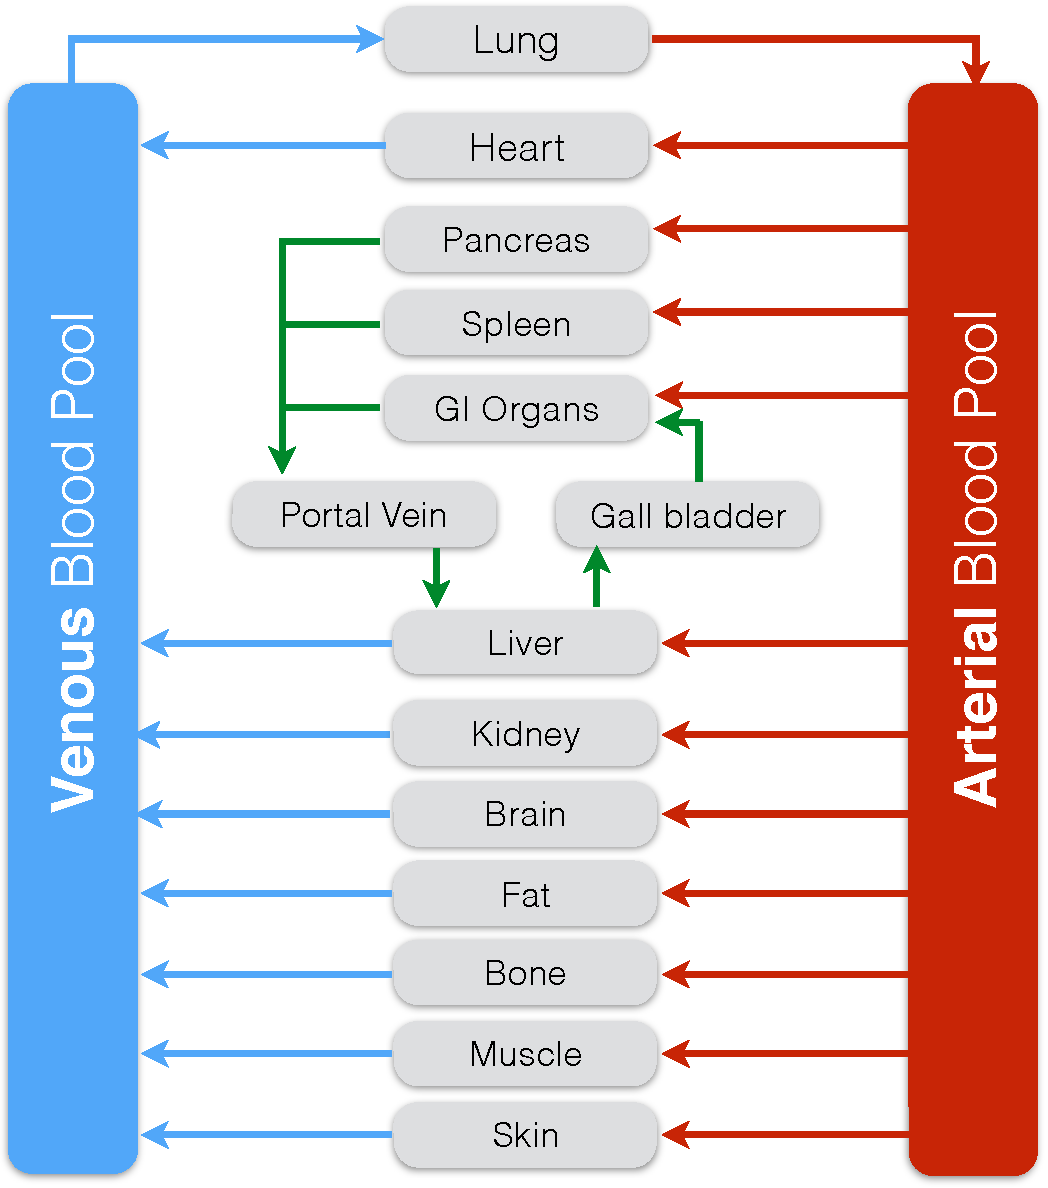
\includegraphics[width=0.29\textwidth]{./figs/PBPK-Figure-7-31-14.pdf}
  \caption{A PBPK with many compartments. Blood flows from the aterial blood pool, through one of the organ compartments, and into the venous blood pool.}\label{fig:SamplePBPK}
\end{wrapfigure}

Current trauma models either simplify the body or the coagulation process.
For example, Ho et al. developed a model that considered blood to be two distinct parts, either hematocrit or plasma, and assumed the rate of fluid loss was the same as the rate of fluid replacement. They did not model the coagulation process; instead, they lumped all of the coagulation factors into one variable, which they correlated with prothrombin time \cite{ho2005mathematical}.
Their model provides guidance on the ratio of fresh frozen plasma (FFP) to packed red blood cells (PRBC) that patients with excessive blood loss should receive.
A slightly more complex model by Hirshberg et al. modeled blood as having three compartments: red cells, plasma, and water, and allowed flow between these compartments based on systolic blood pressure \cite{hirshberg2003minimizing}. They used prothrombin time to quantify if a patient was at risk for dilutional coagulopathy, and did not consider the biological mechanisms behind coagulation. A model without compartments, but containing more physiological functions was developed by Simpson et al. \cite{simpson1996computer}.
Simpson's model allows for both blood pressure and bleed out rate to change over time, with the bleed out rate decreasing as blood pressure decreases. This model predicts hematocrit levels over time, but not the levels of specific proteins. Reisner et al. re-purposed their model of the cardiovascular system (which was originally created to predict how the cardiovascular system responds to orthostatic stress) to study hemodynamic responses to haemorrhage \cite{reisner2013computational}.
Their model includes the heart and pulmonary circulation as well as four peripheral tissue compartments representing the upper body, legs, viscera and kidneys, each of which received the same fraction of the cardiac output. They modeled blood by separating it into two components: red blood cells and plasma.
This model includes transcapillary fluid exchange and lymphatic flow but groups all proteins together.

\subsection*{Modeling of heart rate.}
A key parameter in the PBPK model is cardiac output (CO). Cardiac output is the product of the stoke volume (amount of blood pumped per beat) and the heart rate, which can be modulated by a variety of stimuli. Olufsen and Ottesen have developed several models of heart rate regulation \citep{olufsen2006modeling, ottesen1997modelling,olufsen2008modeling,olufsen2013practical}.
Heart rate is determined, in part, by the sympathetic and parasympathetic nervous system.
Sympathetic nervous system stimulation releases the hormones epinephrine and norepinephirine into the circulation, which increase heart rate.
On the other hand, the parasympathetic system releases acetylcholine which decreases heart rate.
These two systems, often described as an accelerator and a brake, are not independent.
Rather, they interact through second messengers cAMP (cyclic adenosine monophosphate) and cGMP (cyclic guanosine monophosphate) \citep{olshansky2008parasympathetic}.
Heart rate is also influenced by the baroreflex system consisting of baroreceptors, which are tension sensitive nerve endings found in the circulatory system \citep{ottesen1997modelling}.
When baroreceptors sense a pressure change, they modulate in the frequency of nerve activity.
When pressure (and stretch) rapidly increase, so does the baroreceptor firing rate \citep{negative1999reflexes}.
The effect of this signal is not instantaneous, rather, there is a time delay on the order of seconds before the sympathetic and parasympathetic nervous systems respond \citep{ottesen1997modelling}. These models use the baroreflex system and the concentrations of acetylcholine and norepinephire to predict heart rate.
They assume changes in arterial wall stretch are proportionate to filtered blood pressure, $\dot{\bar{p}} = \alpha(-\bar p + p)$
where $\alpha$ is a gain, $\bar p$ is the filtered blood pressure, and $p$ is the patient's measured blood pressure.
From $\bar p$, we can predict the nervous system firing rate, $n = \sum_i n_i + N,~i = 1,2$
where N is a baseline firing rate and $n_i$ corresponds to the firing rate of nerve fibers of type $i$.
The firing rates for nerves of type $i$ are computed as:
\begin{equation}
\frac{dn_i}{dt} = \kappa_i \frac{d \bar p}{dt} \frac{n(M-n)}{(M/2)^2}-\frac{n_i}{\tau_i}, i = 1,2
\end{equation}
where $M$ is the maximum firing rate, and $\tau_i$ is the time scale for nerves of type $i$.
The firing rate information is compiled by the central nervous system, which then determines the the sympathetic and parasympathetic outputs, $f_{sym}$ and $f_{par}$, respectively.
The parasympathetic output is given by $f_{par} = n/M$, while sympathetic output takes the form:
\begin{equation}
f_{sym} = \frac{1-n(t-\tau_d)/M}{1+\beta f_{par}}
\end{equation}
With these outputs, we can determine the dimensionless concentrations of acetylcholine, $c_{ach}$ and noradrenaline, $c_{nor}$:
\begin{equation}
\label{dcnordt}
\frac{dc_{j}}{dt} = \frac{f_{i}-c_{j}}{\tau_{j}}
\end{equation}
where each $\tau_{j}$ represents a time scale.
Finally, the heart rate is calculated from $h_0$, the intrinsic heart rate, and $m_{nor}$ and $m_{ach}$,
which are weights for the contributions of acetylcholine and norepinephrine to heart rate $h = h_0(1+m_{nor}c_{nor} - m_{ach}c_{ach})$.


% \subsection*{Coagulation and Fibrinolysis}
% Historically, the coagulation cascade was considered to be two distinct pathways, the extrinsic and intrinsic, but today, it is known that the two pathways are linked.\cite{adams2009review}
% \subsubsection*{Clot Formation}
% The coagulation process begins when an injury occurs, which exposes tissue factor, a transmembrane protein expressed on the surface of cells surrounding blood vessels. \citep{mackman2009role} The newly exposed tissue factor can then bind to factor VIIa (FVIIa), thus forming the extrinsic tenase complex. Then, the extrinsic tenase complex catalyzes the conversion of FX and FIX to their active forms, FXa and FIXa. \cite{mann2006models} FXa converts a small amount of prothrombin to thrombin, and this thrombin then activates FV, FVIII, and FXIII giving rise to FVa, FVIIIa, FXIIIa.\cite{orfeo2004factor} Thrombin also binds to G-coupled protein receptors on platelet membranes, activating the platelets and inducing them to aggregate.\citep{hoffman2009hematology} FIXa and FVIIIa form the intrinsic factor tenase complex, which strongly converts FX to FXa, leading to a large increase in thrombin production. FXa and FVa bind together to form the prothrombinase complex, which converts prothrombin to thrombin about $10^8$ times efficiently as FXa alone. \cite{walker1994activation} The large amount of thrombin produced leads to the conversion of fibrinogen to fibrin, and FXIIIa helps cross link the fibrin to form a stable network, leading to the formation of a clot. \cite{hoffman2009hematology}
% %Coagulation has been modelled at varying levels of detail. This process has been modelled in great detail using ordinary differential equations, keeping track of 92 proteins and 148 protein-protein interactions, with each reaction modelled using mass action kinetics. \cite{luan2007computationally}  Additionally, it has been modeled as a set of positive feedback loops, with the last loop further activating the first loop.\cite{beltrami1995mathematical} More recently, Varner et al created a reduced order model of coagulation by combining ordinary differential equations with logical rules. \cite{sagar2015dynamic} This reduced order model contains only five differential equations, making it much less computationally intensive to solve.
%
% The clot formation process, with respect to thrombin, is a positive feedback loop with a small amount of thrombin leading to the generation of large amounts. This process can be stopped by several different inhibitors, including one activated thrombin: thrombomodulin. Thrombomodulin inhibits the formation of additional thrombin by binding to thrombin (preventing thrombin from activating any other factors), and the thrombin-thrombomodulin complex activates Protein C. \cite{esmon1989roles} Protein C, with its cofactor protein S, inactivates factors Va and VIIIa. \citep{esmon1987anticoagulation}
% Tissue factor pathway inhibitor stops the clotting process in two ways: it binds to the FVIIa:TF complex, making it unavailable to produce FXa and FIXa, and it binds to already produced FXa, rendering it inactive. \cite{lwaleed2006tissue} Antithrombin binds to active factors, preventing them from further catalyzing the clotting process. \cite{olson1994regulation}  Protein Z complexes with protein Z-dependent protease inhibitor in plasma, and reduces the activity of FXa, FXIa, and FIXa. \citep {corral2007protein}
% Thrombin activated fibrinolysis inhibitor (TAFI) is activated the thrombomodulin-thrombin complex. \citep{chapin2015fibrinolysis}. It removes the lysine and arginine residues form the C-terminal of fibrin, which reduces the number of sites at which plasmiogen can bind, stabilizing the clot.
% \subsection*{Fibrinolysis}
% Fibrinolysis, the process that breaks down clots, must be in balance with coagulation, otherwise, coagulopathy or disseminated intravascular coagulation may occur. Plasmin, the enzyme that breaks down clots, has two activators, tPA and uPA. \cite{wiman1978molecular} Tissue plasminogen activator (tPA) or urokinase (uPA) convert plasminogen, the plasmin precursor, to plasmin on the surface of the clot or on cell membranes. \citep{chapin2015fibrinolysis} Both tPA and uPA are serine proteases and have short half-lives in circulation, on the order of 4-8 minutes, before they are destroyed in the liver. Their locations of manufacture differ: tPA is produced endothelial cells, uPA is produced by monocytes and macrophages. Both are inhibited by plasminogen activator inhibitor-1 (PAI-1), and tPA increases dramatically in activity when it binds fibrin. \citep{chapin2015fibrinolysis}
% \subsection*{Complement}
% Complement, named for its ability to improve the activity of the immune system, also interacts with the coagulation cascade. Complement can be activated by three major pathways: the classical pathway, the lectin pathway, or the alternative pathway. \citep{oikonomopoulou2012interactions} Antigen-antibody complexes trigger the classical pathway, the carbohydrates on the surfaces of microbes initiate the the lectin pathway, and the binding of C3b to properdin or the the spontaneous activation of complement component 3 (C3) by hydrolysis triggers the alternative pathway. All of these pathways intersect with C3 convertase. \citep{markiewski2007complement}
% C3a activates platelets, increasing their tendency to aggregate. C3b is converted into C5 by C3 convertase, resulting in the formation of C5a and C5b. The presence of C5a increases the tendancy of blood to clot by upregulating the production of tissue factor. Although thrombin isn't traditionally included in the compliment pathway, it also plays a role. Thrombin can act on both C3 and C5 to produce C3a,C3b,C5a and C5b, amplifying compliment. \citep{oikonomopoulou2012interactions}
%Bannish created a very detailed model of fibrinolysis using a stochastic model to model tPA binding and combined that with a macrosccale model to measure how fast the lysis front moves. \cite{bannish2012modelling} The dissolution of clots has also been modeled using the Naiver Stokes equation for flow over and through the clots combined with mass balances over the relevant species.\cite{wootton2002experimental}
%\subsection*{Previous Trauma Models}
%Several whole body models of trauma exist, however, they tend to either simplify the body or the coagulation process.
%Ho et al developed a model that considered blood to be two distinct parts, either hematocrit or plasma, and assumed that the rate of fluid loss was the same as the rate as fluid replacement. They did not model any of the dynamics of the coagulation process, rather, they lumped all of the coagulation factors into one variable, which they correlated with prothrombin time. \cite{ho2005mathematical} Their model provides guidance on the ratio of fresh frozen plasma (FFP) to packed red blood cells (PRBC) that patients with excessive blood loss should receive.
%A slightly more complex model by Hirshberg et al modelled blood as having three compartments: red cells, plasma, and water, and allowed flow between these compartments based on systolic blood pressure. \cite{hirshberg2003minimizing} They used prothrombin time to quantify if a patient was at risk for dilutional coagulopathy, and did not consider the biological mechanisms behind coagulation. A model without compartments, but containing more physiological functions was developed by Simpson et al.\cite{simpson1996computer}
%Simpson's model allows for both blood pressure and bleed out rate to change over time, with the bleed out rate decreasing as blood pressure decreases. This model predicts hematocrit levels over time, but not the levels of specific proteins.
%Reisner et al re-purposed their model of the cardiovascular system (which was originally created to predict how the cardiovascular system responds to orthostatic stress) to study hemodynamic responses to haemorrhage.\cite{reisner2013computational} Their model includes the heart and pulmonary circulation as well as four peripheral tissue compartments representing the upper body, legs, viscera and kidneys, each of which received the same fraction of the cardiac output. They modelled blood by separating it into two components: red blood cells and plasma. This model includes transcapillary fluid exchange and lymphatic flow, but groups all proteins together.
%%%%%%%%%%%%%%%%%%%%%%%%%%%%%%%%%%%%%%%%%%%%%%%%%%%%%%%%%%%%%%%%%%%%%
% PRELIMINARY RESULTS
%%%%%%%%%%%%%%%%%%%%%%%%%%%%%%%%%%%%%%%%%%%%%%%%%%%%%%%%%%%%%%%%%%%%%

\section*{Research plan}

\subsection*{Aim 1: Develop a state-aware mathematical model of the human body.}
The objective of this aim is to create a model of the human body with a heart rate and blood pressure that changes with the patient's blood volume. Toward this aim, we have implemented a model that predicts heart rate based on blood pressure. We then optimized the parameters used in this model, which greatly improved the accuracy of the predictions.

\paragraph*{Reduced order modeling of biochemical trauma cascade.}
\begin{wrapfigure}{l}{0.40\textwidth}
  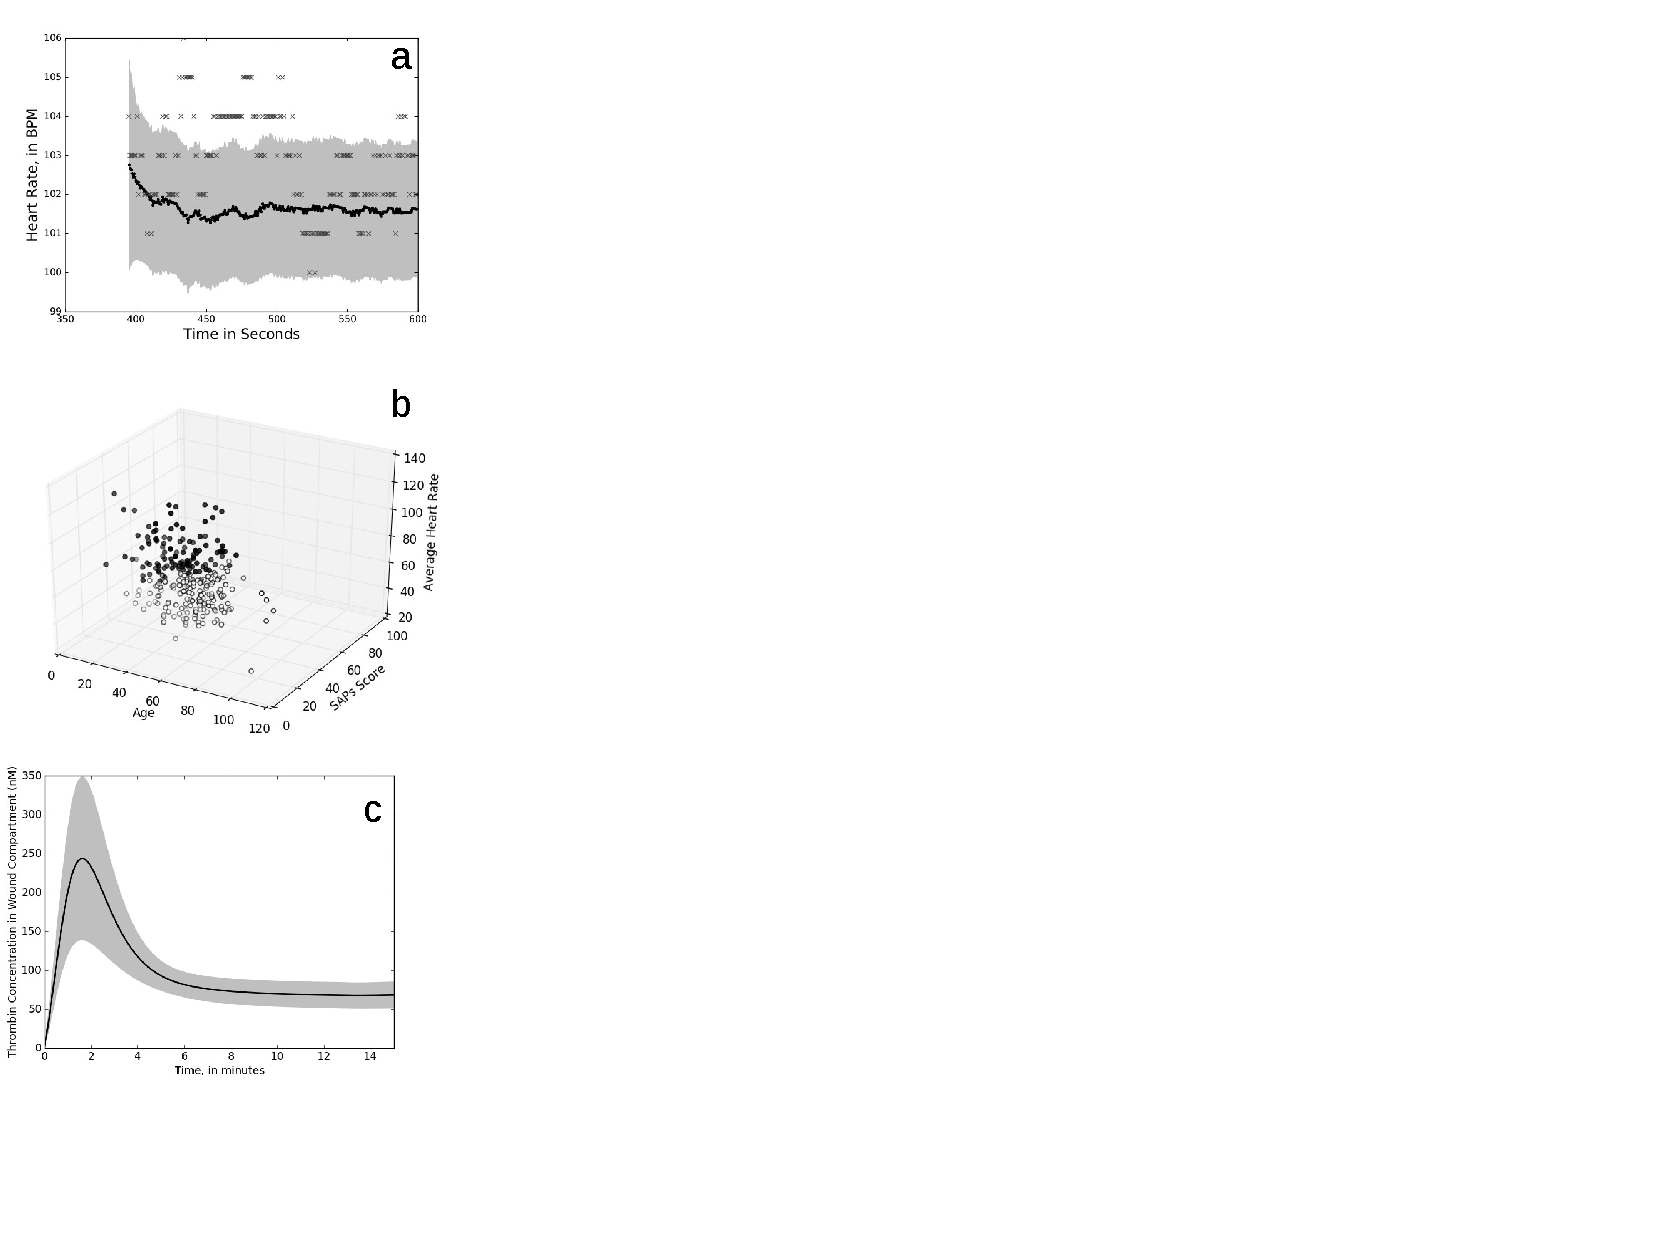
\includegraphics[width=0.39\textwidth,trim={0cm 2cm 20.2cm 0},clip]{./figures/colfigure.pdf}
  \caption{Simulation of heart rate model is shown in subfigure A. The x represent the true data, the black dots represent the average model performance over the 10 different parameter sets, and the grey is a 95\% confidence interval. Subfigure shows the clustering of the MIMIC patients. Subfigure C shows the concentration of thrombin in the wound compartment of the PBPK, with the black being the mean concentration and the grey showing a 95\% confidence interval for collection of patient with different organ volumes and initial concentrations.}\label{fig:mulitobjperformance}
\end{wrapfigure}
A reduced order model of the trauma cascade allows us to capture the essence of the biological processes occurring while reducing the number of differential equations that must be solved. This reduction is useful in PBPK modeling, where the differential equations governing the behaviour of species must be solved in each compartment. 
A reduced order model of fibrinolysis is currently under development by the Varner group. This model expands on the reduced order coagulation model by including 18 species. We will validate the reduced order fibrinolysis model using ROTEM, TEG, and FIIa time series measurements taken at the University of Vermont. Incorporating it into PBPK will allow us to study both coagulopathy and DIC. The larger reduced order model allows us to track more species, providing us with more points of comparison between the model and experimental data, for better estimation of kinetic parameters. The development of a reduced order model of complement, a component of the immune response, is also underway. In its current form, this small model predicted the overall trends of C3a and C5a concentration, but the C3 dynamics were too fast. By changing how tickover (the spontaneous hydrolysis of C3) is described in the model, we can better capture the dynamics of C3 formation.  We will compare the complement model's prediction to experimental data to insure that it accurately describes the dynamics of the system \cite{morad2015time}. Although compliment is a pathway traditionally associated with the immune response, it activated following trauma, and shifts the balances towards coagulation by activating platelets and increasing tissue factor expression \cite{markiewski2007complement}. By including a complement in our trauma model, we will be able to capture the interactions between complement and coagulation, which may prove important to accurately describe DIC. Furthermore, we will be able model platelet activation, as both C3 and C5b-9 alter platelet behavior \cite{peerschke2008platelet}.


\paragraph*{Identification of a heart rate model for trauma patients.}
We estimated heart rate model parameters using 273 patients from the MIMIC-II/III, a freely-available database comprising deidentified health-related data associated with
over forty thousand patients who stayed in critical care units of the Beth Israel Deaconess Medical Center between 2001 and 2012 \cite{Johnson:2016aa}.
When less than 10\% of blood volume has been lost, the barroreflex is initiated as pressure has dropped to increase heart rate \cite{foex1999systemic}.
After approximately 10\% of blood volume has been lost, heart rate begins to decrease, as does blood pressure.
When blood loss approaches 30\% of blood volume, heart rate increases dramatically \cite{jacobsen1990cardiovascular}.
During all three phases, the concentrations of adrenaline, noradrenaline, and vasopressin rise, but then decrease once blood is transfused.
Using the blood pressure tracks from MIMIC II, we used Olufsen's and Ottsen's model \cite{olufsen2013practical} to predict heart rate within the PBPK model.
We used the Nelder Mead algorithm to estimate parameters that better fit the MIMIC II data.
Additionally, we used k-means clustering to group the patients into two clusters, based on age, average heart rate, and SAPS (Simplified Acute Physiology) score.
We then used the JuPOETS multiobjective optimization package \cite{bassen2016jupoets} to generate families of parameters for the two clusters (Fig. \ref{fig:mulitobjperformance}).
The estimated parameters reduced the total mean squared error by more than two-thirds. Furthermore, we used the acetylcholine and noradrenaline concentrations predicted by this model to vasodilate and constrict the arterial and venous blood pools. The aerial and venous blood are constricted if the noradrenaline concentration is above a threshold value, and dilated if the acetylcholine concentration is above a threshold value. The expansion and contraction of the compartments was capped at 125\% and 75\% of their resting values, respectively to prevent unphysical volume changes. The degree of volume change was based on previous experimental data on volume change as a function of a concentration of acetylcholine and noradrenaline \cite{chowienczyk1994blood,dora1983effect}.
In general, adding the heart rate change and vassocative factors to the model slightly shifts the curves, but does not alter their overall shape.

\paragraph*{Incorporating reduced order biochemical models into the PBPK framework.}
We constructed an eight compartment model of the human body, using the Kwatee code generation system \citep{varnerlab_2015_32628}.
In this model, blood flowed from a venous pool, to the heart, through the lungs, back through the heart, and into an arterial blood pool.
Blood then passed from the arteries through the liver, kidney, or bulk to the veins. All of the proteins flowed freely between compartments, except for thrombomodulin and trigger, which are bound to cell membranes \cite{esmon1989roles}. We simulated a small wound connected to the arterial blood pool, with a volume of 0.5\% of the total blood volume. Coagulation dynamics were modeled using the reduced order model constructed by Sagar et al. \cite{sagar2015dynamic}. In the reduced order model, trigger (which biologically corresponds to to the tissue factor-FVIIa complex) activated thrombin. Thrombin then catalyzed its own activation, as well as the activation of Protein C, which inhibited the activation of thrombin. Antithrombin complexed with thrombin and deactivated it. We ran the model in a collection of different patients, each with slightly different organ volumes and initial concentrations, with the thrombin concentration in the wound compartment shown in Figure \ref{fig:mulitobjperformance}c. The patient is bleeding out at a constant rate of 10.5 mL/min, which would lead to complete exsanguination in less than ten hours. As blood volume diminishes, the heart rate of the patient increases.
The blood loss comes from the arterial and bulk compartments, leading to a rise in the concentration of thrombomodulin in those compartments, as their volume is decreasing while the amount of thrombomodulin present remains constant.

% \begin{figure}
% %\begin{wrapfigure}{R}{\textwidth}
%         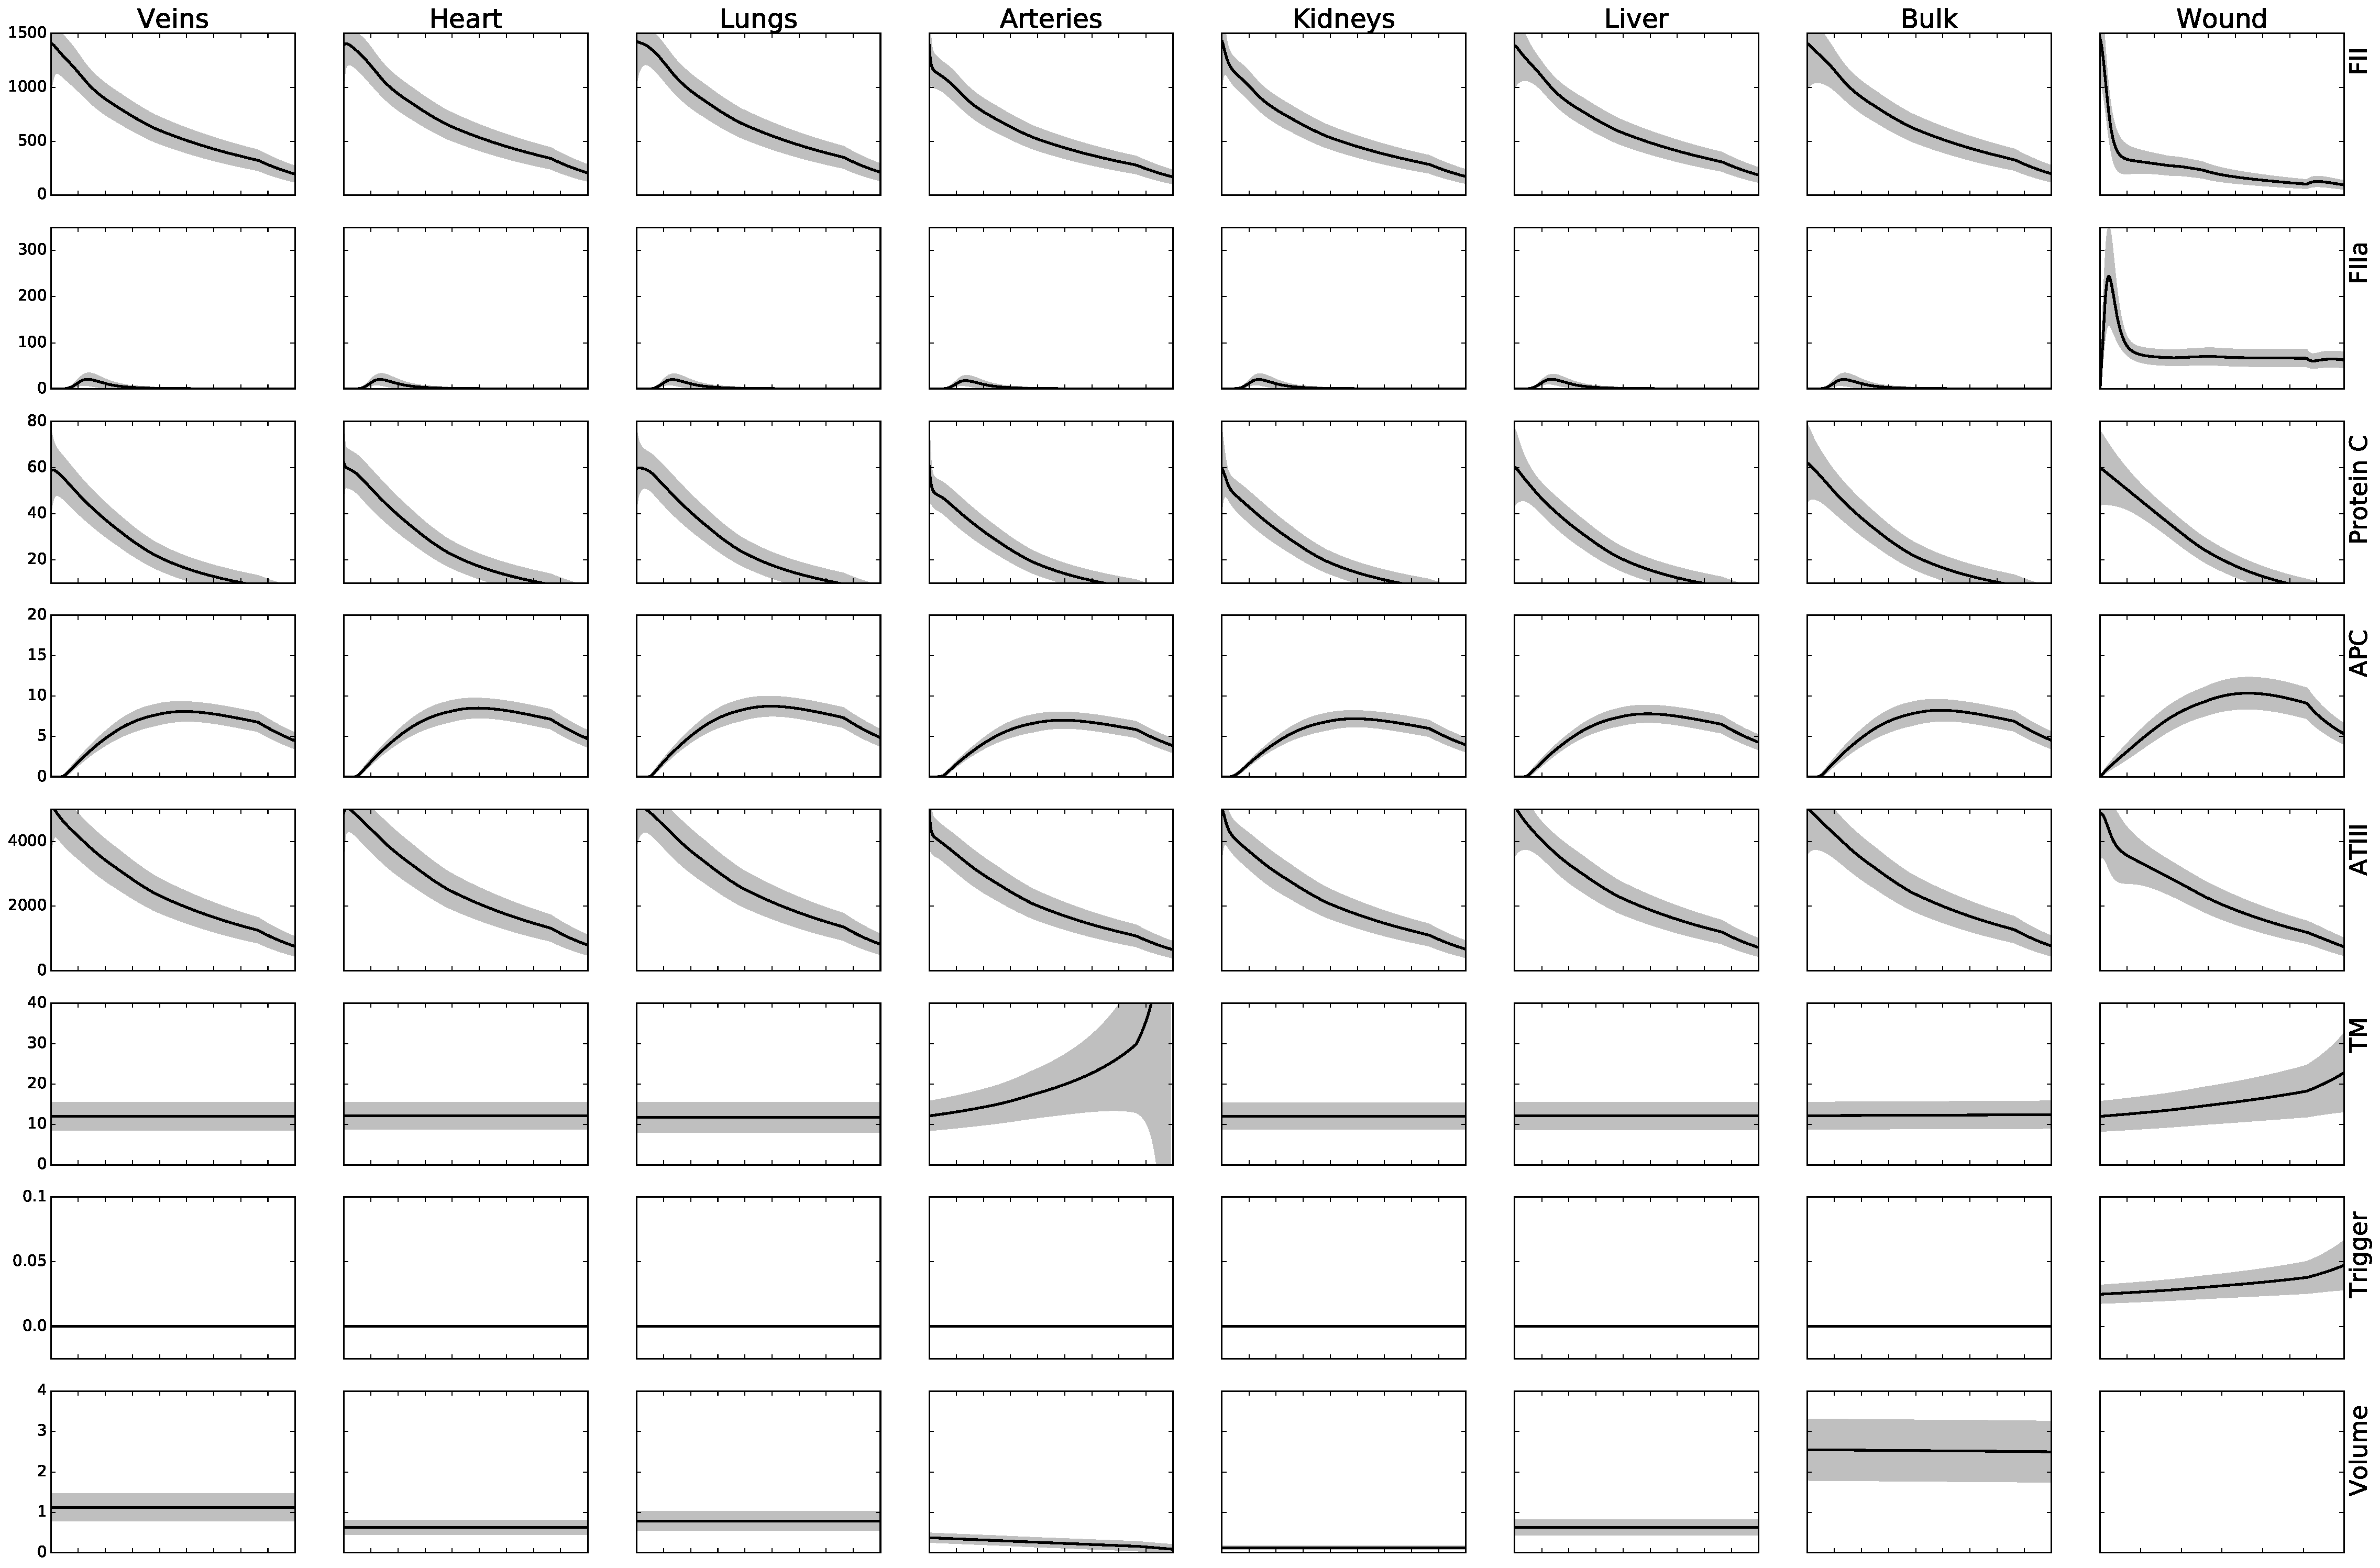
\includegraphics[width=\textwidth]{figures/DifferingInitialVolumesAndConditionsPrettyDiffContraction}
%         \caption{\scriptsize All concentrations given in nanomolar, and times in minutes. Each tick on the x-axis represents five minutes. Volumes are given in liters. The black line represents the average response over 100 patients whose initial concentrations were permitted to vary by up to 25\%, as were their organ volumes. The black line is the average response, and the grey is a 95\% confidence interval.}
%         \label{fig:demoPBPK}
% %\end{wrapfigure}
% \end{figure}


\subsubsection*{Proposed studies.}
With the aim to develop a model of acute haemorrhage and resuscitation, Menezes created a method of estimating blood pressure as a function of the blood volume lost and allowing the bleed out rate to vary as a function of blood pressure  \citep{menezes1998computer}. His model also allows total blood volume to change based on trans-capillary refilling, the process through which fluid moves from interstitial space into the blood due to a change in pressure. We will use his model to predict blood pressure as a function of blood loss, and combine it with the previously described heart rate prediction model to create our state aware body. Johansson et al collected extremely detailed bloodwork on adult trauma patients at a level one trauma center, including thrombin/antithrombin-complexes, antithrombin, protein C, fibrinogen, FXIII levels as well as activated partial thromboplastin time \citep{johansson2011disseminated} approximately one hour after injury. We can compare our model predictions to Johanssons's data to confirm that the model predictions are valid. 

\paragraph*{Expected outcomes, potential pitfalls and alternative approaches.}
We expect Aim 1 will produce  a model body with time varying heart rate and blood pressure with the reduced order models of fibrinolysis, coagulation, and compliment running in each compartment. However, if the reduced order models fail to capture the combined dynamics of coagulation, fibrinolysis, and complement, we can consider alternative, more complex ODE or PDE based models of each process. Should the combination of heart rate and blood pressure models fail to give a sufficient description of the human body, a more complex model, such as the one developed by the SAPHIR project will be implemented \citep{thomas2008saphir}. We expect our approach will be successful, as it will build upon previously proven models.

\subsection*{Aim 2: Develop personalized models of trauma. }
\subsubsection*{Proposed studies.}To capture a spectrum of responses in a model, it is necessary to consider the variation in physiological parameters between individuals. The P$^3$M project has developed a large set of bodies that can be used to test PBPK models \citep{price2003modeling}. This set of bodies includes both organ masses as well as perfusion rates for male and female bodies. We can use this spectrum of bodies to compare coagulation and fibrinolysis in bodies of varying size and composition to see the range of responses and use the correlations developed by the P$^3$M model to generate organ volumes based on the height and weight of individuals.
We also need to capture the biochemical differences between individuals. Studies have associated genes with circulating fibrinogen levels \cite{dehghan2009association}, Protein C levels \cite{russell2003genetics}, activated partial thromboplastin time and prothrombin time \cite{tang2012genetic}, and thrombosis \cite{lane1996inherited}. We can combine this information with the sequences available from the 1000 Genomes project to generate differing initial concentrations and rate constants for individuals. 

\paragraph*{Expected outcomes, potential pitfalls and alternative approaches.} At this point, the model will take in patient physiological data to produce more accurate predictions of how this patient will respond to traumatic injury.  
If the proposed method of using genetic information proves unfeasible, the Plasma Proteome Database includes concentrations of many proteins found in blood plasma and serum \cite{nanjappa2013plasma}. We can use these concentrations as an average, and then generate a distribution of concentrations to simulate the population.
\subsection*{Aim 3: Predict the patient-specific efficacy of trauma interventions.}
\subsubsection*{Proposed studies.}
Current treatment for trauma patients requiring massive transfusion is crystalloids, followed by red blood cells, and then plasma and platelets, but newer military studies have shown that outcomes improve if patients receive plasma and platelets earlier while minimizing the amount of crystalloids \cite{holcomb2008increased}. With our personalized model, we can test to see how patient survival changes under both treatment schemes. We can also examine patient survival if clotting factor concentrates are given, as is currently the treatment in Europe \citep{hunt2014bleeding}.

\paragraph*{Expected outcomes, potential pitfalls and alternative approaches.}
We expect that the outcome of aim 3 will provide support for a fluid treatment schedule and dosage for trauma patients. It may turn out that there is no one universally best treatment, that outcomes are highly dependant on physiological and genetic factors. Although our model will consider both physiological and biological processes, it is possible that its treatment recommendations may differ from those in the literature due to a mechanism not included in the model. If that is the case, and a model for the mechanism is available and easily implementable, it will be included in the model. 


% \subsection*{PBPK With Changing Heart Rate and Volume Changes}
%
%
% \section*{Research Plan}
% \subsection*{Expand Biochemical Details-Aim 1 (Fall 2016-Spring 2017)}
%
%
% \subsection*{Improve Mathematical Body Model-Aims 1 \& 2 (for A exam, Summer 2017-Summer 2018)}
% The present body used in this model is extremely simplistic, consisting of a few well mixed compartments, with constant flow rates between them. It neglects nearly all of the other physiological processes that are a part of traumatic injury, which would be included in a more detailed model. There are very complex models of the human body, some with thousands of parameters, others merely with hundreds. \cite{thomas2008saphir, guyton1972circulation,coleman1983comprehensive} The challenge lies in selecting a model which captures just enough detail to capture the dynamics of the process without making the model unduly complex.
%
% With the aim to develop a model of acute hemorrhage and resuscitation, Menezes created a method of estimating blood pressure as a function of the blood volume lost, and allowing the bleed out rate to vary as a function of blood pressure.\cite{menezes1998computer} His model also allows total blood volume to change based on trans-capillary refilling, the process through which fluid moves from interstitial space into the blood due to a change in pressure. Incorporating his model of blood pressure and blood loss will allow us to more accurately capture the dynamics of traumatic injury.
% Olufsen and Ottesen have developed several models of heart rate as a function blood pressure, however, these models only incorporate the baroreflex and two neurotransmitters.\citep{olufsen2006modeling, ottesen1997modelling,olufsen2008modeling,olufsen2013practical} They fail to capture the longer term (over the scale of hours) dynamics of the cardiovascular system, but this model can be used in conjunction with Meneze's blood pressure model to give the simulated body a dynamic heart rate over the duration of minutes. For longer durations, we can use data recorded in lower body negative pressure tests (a technique used to mimic blood loss) to generate a heart rate based on the the decrease in blood pressure. \cite{mohanty1989neurohumoral,murray1968hemodynamic} Should the combination of these models fail to give a sufficient description of the human body, a more complex model, such as the one developed by the SAPHIR project will be implemented.\cite{thomas2008saphir}
%
% Once the biochemical and physiological modules of the model have been integrated, we can validate the model by comparing its predictions to data recorded in trauma centers or available in MIMIC III.\cite{johansson2011disseminated,johnson2016mimic} MIMIC III provides a wealth of information about patients admitted to the Beth Israel Deaconess Medical Center ICU, however, the amount of information available about each patient varies greatly, depending on what tests were ordered. Since MIMIC III contains information about what treatment options a patient received, we can use this data to insure that the model responds properly to fluid inputs.
%
% Following validation, we can use the model to test how our simulated patient responds to treatment. Current treatment for trauma patients requiring massive transfusion is crystalloids, followed by red blood cells, and then plasma and platelets, but newer military studies have shown that outcomes improve if patients receive plasma and platelets earlier while minimizing the amount of crystalloids. \cite{holcomb2008increased} With our model, we can test to see how clot formation changes under both treatment schemes.
% \subsection*{Population Modeling and Personalization-Aim 3 (Beyond A exam)}
% In an ideal case, we could instantaneously sequence the DNA of the individual and predict how they will respond to various treatments, but science has not yet advanced to that level. Instead, there is a broad spectrum of responses, dependent on many genetic and environmental factors. To capture this spectrum of responses in a model, it is necessary to consider the variation in physiological parameters between individuals.
% The P$^3$M project has developed a large set of bodies that can be used to test PBPK models. \cite{price2003modeling} This set of bodies includes both organ masses as well as perfusion rates for male and female bodies. We can use this spectrum of bodies to see compare coagulation and fibrinolysis in bodies of varying size and composition to see the range of responses and use the correlations developed by the P$^3$M model to generate organ volumes based on the height and weight of individuals.
%
% We also need to capture the biochemical differences between individuals. Studies have associated genes with circulating fibrinogen levels\cite{dehghan2009association}, Protein C levels\cite{russell2003genetics}, activated partial thromboplastin time and prothrombin time\cite{tang2012genetic}, and thrombosis \cite{lane1996inherited}. We can combine this information with the sequences available from 1000 Genomes project to generate differing initial concentrations and rate constants for individuals. If this method proves unfeasible, the Plasma Proteome Database includes concentrations of many proteins found in blood plasma and serum. \cite{nanjappa2013plasma} We can use these concentrations as an average, and then generate a distribution of concentrations to simulate the population.
% \section*{Future Perspectives}
% Traumatic injuries have been with humanity since its beginnings, and will continue to occur for the foreseeable future. Thanks to modern medicine, traumatic injury no longer means certain death. Even though medicine may be able to prevent death from the initial wound, later complications still prove deadly in many cases. The proposed model, and the models that will follow, will help to test interventions that will reduce deaths from trauma related complications. Furthermore, this model will help us to understand how the the different biochemical systems involved in trauma interact and influence survival.

%%%%%%%%%%%%%%%%%%%%%%%%%%%%%%%%%%%%%%%%%%%%%%%%%%%%%%%%%%%%%%%%%%%%%
% OTHER STUFF
%%%%%%%%%%%%%%%%%%%%%%%%%%%%%%%%%%%%%%%%%%%%%%%%%%%%%%%%%%%%%%%%%%%%%
%%%%%%%%%%%%%%%%%%%%%%%%%%%%%%%%%%%%%%%%%%%%%%%%%%%%%%%%%%%%%%%%%%%%%
% BIBLIOGRAPHY
%%%%%%%%%%%%%%%%%%%%%%%%%%%%%%%%%%%%%%%%%%%%%%%%%%%%%%%%%%%%%%%%%%%%%
\clearpage
\bibliography{lecover-q-ref,References_v1}
% \bibliographystyle{ieeetr}
%%%%%%%%%%%%%%%%%%%%%%%%%%%%%%%%%%%%%%%%%%%%%%%%%%%%%%%%%%%%%%%%%%%%%
% Fig.S
%%%%%%%%%%%%%%%%%%%%%%%%%%%%%%%%%%%%%%%%%%%%%%%%%%%%%%%%%%%%%%%%%%%%
\end{document}
